
\documentclass[a4paper,12pt]{scrartcl}
\usepackage[utf8]{inputenc}
\parindent 0pt

%opening
\author{}
\date{}
\title{q-Enumeration}
\usepackage[ngerman]{babel}

\usepackage{amsopn}

\usepackage{amsmath,amsthm,amssymb,amscd,color,graphicx}
\usepackage{multicol}
\usepackage{hyperref}
\usepackage{ulem}
\usepackage{color}
\usepackage{tikz}
\usetikzlibrary{arrows,decorations.pathreplacing}
\usepackage{subfig}

\theoremstyle{definition}
\newtheorem{defn}{Definition}
\newtheorem{bsp}[defn]{Beispiel}

\theoremstyle{plain}
\newtheorem{prop}[defn]{Proposition}
\newtheorem{satz}[defn]{Satz}

\theoremstyle{remark}
\newtheorem{bem}[defn]{Bemerkung}
\newtheorem{aufg}[defn]{Aufgabe}
\newtheorem{tipp}[defn]{Tipp}
\newtheorem{motto}[defn]{Motto}


\newcommand{\NN}{\mathbb{N}}
\newcommand{\RR}{\mathbb{R}}
\newcommand{\Slope}{S}
\newcommand{\Front}{F}
\newcommand{\Intersect}{\Delta}


\begin{document}

 \begin{picture}(0,0)
  \put(0,-15.5){
   
\includegraphics[scale=0.1]{logo-ifm}
  }
  \put(400.0,-100.){
   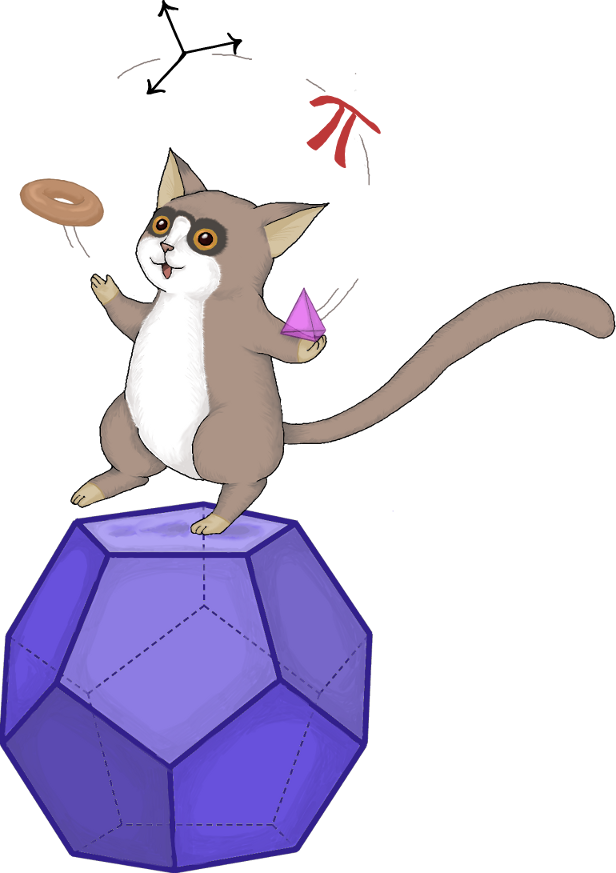
\includegraphics[scale=0.17]{cover}
  }
 \end{picture} 

 \vspace{6em}
 
 \section{Problem}
  
  Mir fehlt hier noch ein guter Aufh\"anger...
  
  \begin{defn}
   Eine Partition einer nat\"urlichen Zahl $n$ ist ein Tupel $(n_1, n_2, \dots, n_k)$ von nat\"urlichen Zahlen mit $n_1  \geq n_2 \geq \dots \geq n_k > 0$ sodass $n_1 + n_2 + \dots + n_k = n$. Jedes $n_i$ in einer solchen Partition hei{\ss}t Teil der Partition.  Man sagt, dass $(n_1, n_2, \dots, n_k)$ eine Partition von $n$ in $k$ Teile ist.\\
   Mit $p(n)$ bezeichnen wir die Anzahl der verschiedenen Partitionen einer nat\"urlichen Zahl $n$. Die Funktion $p \colon \NN \to \NN, n \mapsto p(n)$, hei{\ss}t die Partitionsfunktion.
  \end{defn}
  
  \begin{motto}
   Eine Partition von $n$ ist eine M\"oglichkeit die Zahl $n$ als Summe von positiven nat\"urlichen Zahlen $n_1, n_2, \dots, n_k$ zu schreiben, wobei Summen, die sich nur in ihrer Reihenfolge der Summanden unterscheiden, als gleich angesehen werden.
  \end{motto}

  \begin{bsp}
   Als Beispiel listen wir mal alle $11$ Partitionen von $6$ auf:
   \begin{multicols}{3}
    \begin{itemize}
     \item[] $(6)$
     \item[] $(5,1)$
     \item[] $(4,2)$
     \item[] $(4,1,1)$
     \item[] $(3,3)$
     \item[] $(3,2,1)$
     \item[] $(3,1,1,1)$
     \item[] $(2,2,2)$
     \item[] $(2,2,1,1)$
     \item[] $(2,1,1,1,1)$
     \item[] $(1,1,1,1,1,1)$.
     \item[]
    \end{itemize}
   \end{multicols}
  \end{bsp}

  Einzelne Partitionen sind f\"ur uns eher uninteressant. Wir interessieren uns daf\"ur umso mehr um die Anzahl $p(n)$ von Partitionen einer beliebigen nat\"urlichen Zahl $n$. Wie Du Dir vorstellen kannst, w\"achst diese Anzahl sehr schnell an. Hier ein paar Beispielswerte: $p(10) = 42$, $p(20) = 627$, $p(30) = 5604$, $p(40) = 37 \, 338$ und $p(100) = 190 \, 569 \, 292$. Die Anzahl der Partitionen der Zahl $10\,000$ hat bereits $107$ Stellen und die Anzahl der Partitionen der Zahl $1\,000\,000$ hat $1108$ Stellen. Zum Vergleich: Es wird vermutet, dass die Anzahl der Atome im Universum etwa $80$ bis $100$ Stellen hat. L\"acherlich wenig sozusagen...\\
  An sich ist es nicht schwer, $p(n)$ durch Auflisten aller Partitionen von $n$ herauszufinden, aber aufgrund der gewaltigen Anzahl an M\"oglichkeiten ist dieser Ansatz praktisch nicht durchf\"uhrbar. Gibt es andere M\"oglichkeiten? Die Antwort ist gl\"ucklicherweise ja! Die drei genialen Mathematiker Hardy, Ramanujan und Rademacher fanden folgende Formel:
  $$
   p(n) = \cfrac{1}{\pi \sqrt{2}} \, \sum_{k=1}^\infty A_k(n) \ \sqrt{k} \ \cfrac{d}{dn} \! \! \left( \cfrac{\sinh \! \left(\cfrac{\pi}{k} \ \sqrt{\frac{2}{3} \left(n - \frac{1}{24} \right)}\right)}{\sqrt{n - \frac{1}{24}}} \right),
  $$
  wobei
  $$
   A_k(n) = \sum_{h=1}^{k} \delta_{gcd(h,k), 1} \ \exp \! \left( \pi i \sum_{j=1}^{k-1} \frac{j}{k} \left(\frac{hj}{k} - \left\lfloor \frac{hj}{k} \right\rfloor -\frac{1}{2} \right) - \frac{2 \pi i h n}{k} \right).
  $$
  Wow! Bei dieser Formel k\"onnen wir nur gemeinsam Staunen, denn leider verstehen auch wir Zirkelleiter diese Formel nicht. Alleine dar\"uber, wie man mithilfe dieser Formel geschickt einen Wert berechnet, haben Mathematiker ganze Arbeiten geschrieben.\\
  
  Es gibt aber noch einen anderen Weg, den wir auch nachvollziehen k\"onnen: Wir k\"onnen Rekursionen herleiten, mit deren Hilfe wir aus uns bereits bekannten Werten der Partitionsfunktion neue Werte mit relativ wenig Aufwand berechnen k\"onnen. Bevor es die Formel von Hardy, Ramanujan und Rademacher gab, war diese M\"oglichkeit die einzige praktikable, gr\"o{\ss}ere Werte der Partitionsfunktion zu berechnen. Der Nachteil dieser Methode ist, wie wir sehen werden, dass man alle (zumindest viele) kleineren Werte der Partitionsfunktion kennen muss, bevor man den n\"achsten berechnen kann. Das soll uns aber nicht st\"oren.

 \section{Herleitung von Rekursionsformeln}
  
  Was jetzt kommt, hat auf den ersten Blick rein gar nichts mit unserer Fragestellung zu tun: Wir multiplizieren mal
  \footnotesize
  $$
   P(X) := (1 + X + X^2 + \dots + X^i + \dots)(1 + X^2 + X^4 + \dots + X^{2j} + \dots)(1 + X^3 + X^6 + \dots + X^{3k} + \dots) \cdots
  $$
  \normalsize
  aus. Vorsicht: 
  Dieses Produkt hat unendlich viele Faktoren und jeder Faktor wiederum endlich viele Summanden. Das ist vielleicht ungew\"ohnlich, aber wir k\"onnen ganz normal damit rechnen. Wir k\"onnen nat\"urlich nie komplett ausmultiplizieren, aber wir k\"onnen durchaus die ersten Koeffizienten berechnen:
  \begin{align*}
   P(X) =  1 + X + 2X^2 + 3X^3 + 5X^4 + \dots
  \end{align*}
  Schauen wir uns mal ganz genau an, wie wir oben den Koeffizienten vor $X^4$ berechnen: Zu diesem erhalten wir wie Du wei{\ss}t einen Beitrag, wenn wir aus dem ersten Faktor $X^4$ und aus allen anderen $1$ ausw\"ahlen, oder wenn wir aus dem ersten Faktor $X$, aus dem dritten $X^3$ und aus allen anderen $1$ ausw\"ahlen und so weiter. Zur besseren \"Ubersicht hier eine Tabelle mit allen  M\"oglichkeiten:\\
  
  $\begin{array}{c|c|c|c|c}
   \text{$1$. Faktor} & \text{$2$. Faktor} & \text{$3$. Faktor} & \text{$4$. Faktor} & \text{alle anderen Faktoren}\\
   \hline
   X^4 & 1 & 1 & 1 & 1 \\
   X^2 & X^2 & 1 & 1 & 1 \\
   X & 1 & X^3 & 1 & 1 \\
   1 & X^4 & 1 & 1 & 1 \\
   1 & 1 & 1 & X^4 & 1
  \end{array}$\\[\baselineskip]
  
  Wie Du siehst, steht in der letzten Spalte immer nur eine $1$, da die Exponenten aller anderen $X$-Potenzen in diesen Faktoren schon zu gro{\ss} sind.\footnote{ Das ist \"ubrigens der Grund, warum wir so gut mit diesem Produkt umgehen k\"onnen. Zwar ist das Produkt \glqq unendlich lang\grqq\ \!, aber f\"ur jeden einzelnen Koeffizienten in der ausmultiplizierten Form brauchen wir nur endlich viele Faktoren zu beachten.} Wir k\"onnen uns also auf die ersten $4$ Faktoren konzentrieren. Wenn wir nur die ersten vier Faktoren ausmultiplizieren, so haben die Exponenten $k$ in der ausmultiplizierten Form folgende Gestalt:
  $$
   k = 1 k_1 + 2 k_2 + 3 k_3 + 4 k_4
  $$
  Dabei ist $k_i$ der Exponent der $X$-Potenz, welche wir im $i$-ten Faktor gew\"ahlt haben.\footnote{ Die $1$ sehen wir dabei als $X^0$ an.}
  Wir suchen speziell nach solchen Kombinationen, sodass der Exponent gleich $4$ ist, wir erhalten also die Gleichung
  $$
   4 = 1 k_1 + 2 k_2 + 3 k_3 + 4 k_4.
  $$
  Wir m\"ussen also passende Werte f\"ur die $k_i$ finden. Jetzt kommt der Clou: Jede solche L\"osung entspricht einer Partition der Zahl $4$. Wir k\"onnen n\"amlich $k_i$ auch als Anzahl der Teile der Gr\"o{\ss}e $i$ sehen. Da die $k_i$ eine L\"osung der Gleichung sind, summieren sich die Teile dann genau zu $4$. Zeit f\"ur ein konkretes Beispiel: Aus
  $$
   4 = 1 \cdot 1 + 2 \cdot 0 + 3 \cdot 1 + 4 \cdot 0
  $$
  erhalten wir die Partition der $4$ mit einem Teil der Gr\"o{\ss}e $1$ und mit einem Teil der Gr\"o{\ss}e $3$, also $4 = 3 + 1$ bzw. $(3,1)$ in der ganz korrekten Tupelschreibweise. In der Tabelle ist eine \"Ubersicht \"uber alle Partitionen der $4$.\\
  
  $\begin{array}{c|c|c|c|c|r}
   \text{$1$. Faktor} & \text{$2$. Faktor} & \text{$3$. Faktor} & \text{$4$. Faktor} & (k_1,k_2,k_3,k_4) & \text{Partition}\\
   \hline
   X^4 & 1 & 1 & 1 & (4,0,0,0) & 1+1+1+1\\
   X^2 & X^2 & 1 & 1 & (2,1,0,0) & 2+1+1\\
   X & 1 & X^3 & 1 & (1,0,1,0) & 3+1\\
   1 & X^4 & 1 & 1 & (0,2,0,0) & 2+2\\
   1 & 1 & 1 & X^4 & (0,0,0,1) & 4
  \end{array}$\\[\baselineskip]
  
  % Nur zur H\"alfte ausf\"ullen und den Rest als Aufgabe?
  
  Wir erhalten nat\"urlich auch f\"ur andere Zahlen als die $4$ Partitionen. Wenn wir Partitionen f\"ur $n$ auf diese Art und Weise finden wollen, k\"onnen wir uns auf die ersten $n$ Faktoren von $P(X)$ beschr\"anken und erhalten Gleichungen der Form
  $$
   n = 1 k_1 + 2 k_2 + 3 k_3 + \dots + n k_n.
  $$
  
  Das Tolle dabei: Wir lassen keine Partition aus, erhalten auf diese Weise also wirklich jede Partition! Gleichzeitig erhalten wir jede Partition nur genau einmal. Was bedeutet das f\"ur den Koeffizienten vor $X^n$ in $P(X)$? Dieser ist nichts anderes als $p(n)$, die Anzahl der Partitionen von $n$, d.\,h.
  $$
   P(X) = p(0) + p(1)X + p(2)X^2 + p(3)X^3 + \dots
  $$
  Wenn wir also wissen wollen, wie viele Partitionen die Zahl $10$ hat, k\"onnen wir einfach beginnen, die ersten $10$ Faktoren von $P(X)$ auszumultiplizieren und uns anschlie{\ss}end ansehen, welcher Koeffizient vor $X^{10}$ steht, das ist die Antwort. Das ist aber noch nicht zufriedenstellend, denn kein Mensch hat Lust ein solch un\"ubersichtliches Produkt zu berechnen.\\ Man nennt $P(X)$ auch die erzeugende Funktion der Partitionsfunktion. Das ist aber nicht so zu verstehen, dass wir in diese erzeugende Funktion $P(X)$ irgendwelche Werte f\"ur $X$ einsetzen m\"ochten, das ergibt in den meisten F\"allen \"uberhaupt keinen Sinn. Man kann sich eine solche erzeugende Funktion eher als W\"ascheleine vorstellen, an der man die Folgenglieder einer Folge der Reihe nach neben den Potenzen einer Variable aufh\"angt, so wie wir es (unbewusst) auch getan haben. Die Potenzen dieser Variable haben keine Bedeutung, sie helfen uns nur, den \"Uberblick zu behalten und sorgen f\"ur Ordnung auf der Leine. Das verbl\"uffende ist, dass man mit erzeugenden Funtionen sinnvolle Ergebnisse \"uber die Folge herausfinden kann, indem man einfach mit ihr rechnet, als w\"are sie eine gew\"ohnliche Funktion. Dabei hat man oft kein ein Gef\"uhl daf\"ur, was diese Rechenoperationen auf der Folge direkt f\"ur Auswirkungen haben. Genau das werden wir jetzt auch machen.\\
  
  Betrachten wir den $m$-ten Faktor von $P(X)$. Die Multiplikation von diesem mit $(1-X^m)$ liefert:
  \begin{align*}
   &(1 + X^m + X^{2m} + X^{3m} + X^{4m} + \dots ) (1 - X^m) \\
   = &(1 + X^m + X^{2m} + X^{3m} + X^{4m} + \dots ) - (X^m + X^{2m} + X^{3m} + X^{4m} + X^{5m} \dots )
   = 1.
  \end{align*}
  Das erm\"oglicht es uns, diesen Faktor sehr kompakt zu schreiben, indem wir einfach durch $(1-X^m)$ teilen:
  $$
   (1 + X^m + X^{2m} + X^{3m} + X^{4m} + \dots ) = \cfrac{1}{1 - X^m}.
  $$
  Wenn wir das f\"ur jeden Faktor von $P(X)$ machen, k\"onnen wir
  $$
   P(X) = \cfrac{1}{(1-X)(1-X^2)(1-X^3) \cdots}
  $$
  schreiben. Das scheint uns erst mal nichts zu bringen. Doch Leonhard Euler entdeckte einen Zusammenhang zwischen dem Nenner $(1-X)(1-X^2)(1-X^3) \cdots$ von $P(X)$ und den sogenannten Pentagonalzahlen, die Du vielleicht schon mal kennen gelernt hast. Durch Ausnutzung dieses Zusammenhangs k\"onnen wir uns dann endlich Rekursionsformeln herleiten. Zun\"achst sollten wir aber kl\"aren, was Pentagonalzahlen \"uberhaupt sind.
  
  \begin{defn}\textbf{Pentagonalzahlen}\\
   Als Pentagonalzahlen bezeichnen wir nat\"urliche Zahlen  der Form
   $$
    n = \frac{k(3k \pm 1)}{2}
   $$
   f\"ur ein $k$, wobei $\pm$ entweder f\"ur $+$ oder f\"ur $-$ steht.\footnote{ Es handelt sich tats\"achlich immer um eine nat\"urliche Zahl und nicht um einen Bruch.: Wenn $k$ gerade ist, ist das klar. Ansonsten ist aber $3k \pm 1$ gerade, und somit ist $n$ auch in diesem Fall eine nat\"urliche Zahl.} Oft werden die Zahlen der Form $\frac{k(3k - 1)}{2}$ als \glqq echte \grqq\ Pentagonalzahlen bezeichnet, w\"ahrend die Zahlen der Form $\frac{k(3k + 1)}{2}$ als erweiterte Pentagonalzahlen bezeichnet werden. Die Folge der echten Pentagonalzahlen beginnt mit $0,\,1,\,5,\,12,\,22,\dots$, die der erweiterten Pentagonalzahlen mit $0,\,2,\,7,\,15,\,26,\dots$. Das folgende Bild erkl\"art die Herkunft des Namens f\"ur die echten Pentagonalzahlen.
   \begin{center}
    % http://www.icoachmath.com/math_dictionary/pentagonal_number.html
    % Erw\"ahnen?
    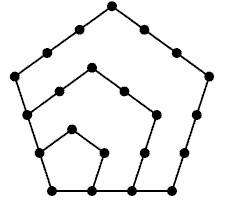
\includegraphics[width=4.5cm,scale=0.8]{Pentagonal_Numbers.jpg}
   \end{center}
   Z\"ahle doch mal, aus  wie vielen Punkten die einzelnen regelm\"a{\ss}igen F\"unfecke (= Pentagon) bestehen. Richtig, aus $1,\,5,\,12,\,22,\dots$ Punkten.
  \end{defn}

  \begin{satz}\textnormal{\textbf{Eulerscher Pentagonalsatz}}\\
  Es gilt
  $$
   (1-X)(1-X^2)(1-X^3) \cdots = 1 + \sum_{k=1}^{\infty} (-1)^k \Big(X^{k(3k+1)/2} + X^{k(3k-1)/2}\Big).
  $$
  Beachte: Die Exponenten auf der rechten Seite sind gerade die Pentagonalzahlen.
  \end{satz}
  
  \begin{proof}
   Der erste Schritt zum Durchblick ist es, eine geeignete Interpretation f\"ur die linke Seite der Gleichung zu finden. Wir wollen schlie{\ss}lich irgendwie wieder zu unseren Partitionen kommen. Wir k\"onnen uns nochmal das Produkt
   $$
    (1 + X + X^2 + \dots + X^i + \dots)(1 + X^2 + X^4 + \dots + X^{2j} + \dots)(1 + X^3 + X^6 + \dots + X^{3k} + \dots) \cdots
   $$
   betrachten, wo wir bereits einen solchen Zusammenhang herstellen konnten. Die Wahl des $i$-ten Summanden im $j$-ten Faktor entsprach in der zugeh\"origen Partition der Wahl von $i-1$ Teilen der Gr\"o{\ss}e $j$. Im Produkt (wir ignorieren erstmal die Minuszeichen)
   $$
    (1+X)(1+X^2)(1+X^3) \cdots
   $$
   haben wir pro Faktor immer nur zwei Summanden zur Auswahl. F\"ur die dadurch beschriebenen Partitionen hei{\ss}t das, dass wir zu jeder Gr\"o{\ss}e entweder kein Teil oder genau ein Teil aufnehmen k\"onnen, nicht aber mehrere. Das bedeutet, dass wir so nur Partitionen beschreiben, die aus lauter verschieden gro{\ss}en Teilen bestehen. Als erzeugende Funktion geschrieben:
   $$
    (1+X)(1+X^2)(1+X^3) \cdots = p_{dist}(0) + p_{dist}(1)X + p_{dist}(2)X^2 + p_{dist}(3)X^3 + \dots,
   $$
   wobei $p_{dist}(n)$ die Anzahl der Partitionen von $n$ in verschieden gro{\ss}e Teile ist.\footnote{ Zum Beispiel hat die Zahl $4$ genau zwei solche Partitionen, n\"amlich $(3,1)$ und $(4)$. Bei allen anderen Partitionen $(1,1,1,1)$, $(2,1,1)$ und $(2,2)$ der $4$ dagegen treten einige Teile gleicher Gr\"o{\ss}e mehrfach auf.} Wenn wir das verstanden haben, k\"onnen wir auch \"uber die Minuszeichen in
   $$
    (1-X)(1-X^2)(1-X^3) \cdots
   $$
   nachdenken: Das Vorzeichen eines Koeffizienten in der ausmultiplizierten Form ist abh\"angig von der Anzahl der Teile der beschriebenen Partition. So erhalten die Terme, die zu Partitionen mit gerade vielen Teilen korrespondieren, positives Vorzeichen, w\"ahrend die Terme, die Partitionen mit ungerader Teileanzahl beschreiben, negatives Vorzeichen erhalten. \"Uberlege Dir das an ein paar Beispielen. Wir erhalten
   $$
    (1-X)(1-X^2)(1-X^3) \cdots = p_{dist}^{g-u}(0) + p_{dist}^{g-u}(1)X + p_{dist}^{g-u}(2)X^2 + p_{dist}^{g-u}(3)X^3 + \cdots,
   $$
   wobei $p_{dist}^{g-u}(n)=p_{dist}^{g}(n) - p_{dist}^{u}(n)$ die Anzahl der Partitionen von $n$ in verschieden gro{\ss}e Teile mit gerader Anzahl von Teilen minus die Anzahl der Partitionen von $n$ in verschieden gro{\ss}e Teile mit ungerader Anzahl von Teilen ist.\\
   Wir werden sehen, dass $p_{dist}^{g-u}(n) \in \{-1, 0 ,1\}$ f\"ur alle $n$ ist, und dass $p_{dist}^{g-u}(n) \neq 0$ nur gilt, wenn $n$ eine Pentagonalzahl ist. Dazu ben\"otigen wir Ferrers Diagramme, die Partitionen visualisieren.
   
   \begin{defn}\textbf{Ferrers Diagramme}\\
    Ein Ferrer Diagramm zu einer Partition $(n_1, n_2, \dots, n_k)$ von $n$ ist ein S\"aulendiagramm mit $k$ S\"aulen, wobei die $i$-te S\"aule $n_i$ K\"astchen hoch ist. Wir veranschaulichen dies mal anhand der Partitionen $(8,7,6,6,5,3)$ und $(8,7,6,5,4,3)$ der Zahlen $35$ und $30$:\\
    
    \begin{figure}[h]
    \centering
    \scalebox{0.5}{
     \begin{tikzpicture}
      %% Markierung
      \draw[fill=red] (0,7) rectangle (1,8);
      \draw[fill=red] (1,6) rectangle (2,7);
      \draw[fill=blue] (5,0) rectangle (6,3);

     % Achsenbeschriftungen
      %\foreach \x in {0,1,2,3,4,5} \foreach \y in {9,8,7,4,3,1} \fill[color=black] (\x,\y) -- (0pt,0pt)
      \draw[color=black] (0,0) grid (1,8);
      \draw[color=black] (1,0) grid (2,7);
      \draw[color=black] (2,0) grid (3,6);
      \draw[color=black] (3,0) grid (4,6);
      \draw[color=black] (4,0) grid (5,5);
      \draw[color=black] (5,0) grid (6,3);
      
      %% Markierung
      \draw[fill=red] (15,7) rectangle (16,8);
      \draw[fill=red] (16,6) rectangle (17,7);
      \draw[fill=red] (17,5) rectangle (18,6);
      \draw[fill=red] (18,4) rectangle (19,5);
      \draw[fill=red!65!blue] (19,3) rectangle (20,4);
      \draw[fill=blue] (19,0) rectangle (20,3);
     
      %% Diagramm
      \draw[color=black] (15,0) grid (16,8);
      \draw[color=black] (16,0) grid (17,7);
      \draw[color=black] (17,0) grid (18,6);
      \draw[color=black] (18,0) grid (19,5);
      \draw[color=black] (19,0) grid (20,4);
     \end{tikzpicture}}
    \end{figure}
    
    Die K\"astchen der $k$-ten (letzten) S\"aule nennen wir Front (im Bild blau markiert). Die jeweils obersten K\"astchen der ersten S\"aulen, sodass die jeweils folgende S\"aule genau ein K\"astchen niedriger ist, werden ebenfalls zusammengefasst. Diese werden wir als Schr\"age bezeichnen. Im Bild sind diese K\"astchen rot markiert. Es kann sein, dass sich die Front und die Schr\"age ein K\"astchen teilen, wie das lila farbene K\"astchen bei der rechts abgebildeten Partition.\\
    Die Anzahl der K\"astchen der Front, der Schr\"age bzw. des Schnitts werden wir mit $\Front$, $\Slope$ bzw. $\Intersect$ abk\"urzen.
   \end{defn}

   
   Wir halten zun\"achst einige kleine Beobachtungen fest: Eine Partition von $n$ ist genau dann eine Partition in verschieden gro{\ss}e Teile, wenn alle S\"aulen im zugeh\"origen Ferrers Diagramm unterschiedlich hoch sind. Ferner ist die Anzahl der K\"astchen des Ferrers Diagramm gleich $n$. Au{\ss}erdem ist $\Intersect = 0$ oder $\Intersect = 1$, d.\,h. die Front und Schr\"age k\"onnen sich maximal ein K\"astchen teilen. Die Anzahl der K\"astchen der Schr\"age ist kleiner gleich der Anzahl der S\"aulen $k$, d.\,h. $\Slope \leq k$ und Gleichheit tritt genau dann auf, wenn $\Intersect = 1$.\\
   
   Wie k\"onnen uns diese Diagramme nun weiterhelfen? Zur Erinnerung: Wir wollten herausfinden, was $p_{dist}^{g-u}(n) = p_{dist}^{g}(n) - p_{dist}^{u}(n)$ ist. Wir werden uns also nur Ferrers Diagramme mit unterschiedlich hohen S\"aulen ansehen. Wir k\"onnten nun versuchen $p_{dist}^{g}(n)$ und $p_{dist}^{u}(n)$ seperat zu berechnen und danach die Differenz bilden. Wir werden anders verfahren.\\
   
   Unser Trick wird sein, soweit m\"oglich zu versuchen, jeder Partition $p$ von $n$ in verschieden gro{\ss}e Teile eine \glqq Partner\grqq\ \!-Partition $p^*$ von $n$ zuzuordnen, die ebenfalls nur aus verschieden gro{\ss}en Teilen besteht. Dabei soll genau eine der verpartnerten Partitionen $p$ und $p^*$ ungerade viele Teile besitzen und die andere entsprechend gerade viele Teile haben. Au{\ss}erdem soll der Partner von $p^*$ wieder $p$ sein (verpartnerte Partitionen sind sich treu), d.\,h. $\left(p^*\right)^* = p$. Wie im echten Leben werden einige Partitionen keinen Partner finden, aber die meisten Partitionen werden nicht alleine bleiben.\\
   
   Was wird uns das bringen? Wir m\"ussen zu einer Zahl $n$ nur wissen, wie viele Partitionen von $n$ partnerlos bleiben. Denn von einem Partitionen-Paar $(p,p^*)$ tr\"agt genau eine Partition zu $p_{dist}^{g}(n)$ und die andere zu $p_{dist}^{u}(n)$ bei. Zusammen genommen wird das Paar also keinen Beitrag zur Differenz $p_{dist}^{g-u}(n) = p_{dist}^{g}(n) - p_{dist}^{u}(n)$ leisten.\\
   
   Wir werden die gesuchte Zuordnung nun am Beispiel der Partition $p = (11,10,9,8,6,5,3)$ von $52$ motivieren. Wie wir anhand des zugeh\"origen Ferrers Diagramm leicht ablesen k\"onnen, ist die Front hier kleiner als die Schr\"age:\\
   
   \begin{figure}[h]
    \centering
    \scalebox{0.5}{
    \begin{tikzpicture}
     %% Markierung
     \draw[fill=red] (0,10) rectangle (1,11);
     \draw[fill=red] (1,9) rectangle (2,10);
     \draw[fill=red] (2,8) rectangle (3,9);
     \draw[fill=red] (3,7) rectangle (4,8);
     \draw[fill=blue] (6,0) rectangle (7,3);
     
     %% Diagramm
     \draw[color=black] (0,0) grid (1,11);
     \draw[color=black] (1,0) grid (2,10);
     \draw[color=black] (2,0) grid (3,9);
     \draw[color=black] (3,0) grid (4,8);
     \draw[color=black] (4,0) grid (5,6);
     \draw[color=black] (5,0) grid (6,5);
     \draw[color=black] (6,0) grid (7,3);
     

     %% Markierung
     \draw[fill=red] (15,10) rectangle (16,11);
     \draw[fill=red] (16,9) rectangle (17,10);
     \draw[fill=red] (17,8) rectangle (18,9);
     \draw[fill=red] (18,7) rectangle (19,8);
     \draw[fill=blue] (15,11) rectangle (16,12);
     \draw[fill=blue] (16,10) rectangle (17,11);
     \draw[fill=blue] (17,9) rectangle (18,10);
     \draw[fill=green] (20,0) rectangle (21,5);
     
     %% Diagramm
     \draw[color=black] (15,0) grid (16,12);
     \draw[color=black] (16,0) grid (17,11);
     \draw[color=black] (17,0) grid (18,10);
     \draw[color=black] (18,0) grid (19,8);
     \draw[color=black] (19,0) grid (20,6);
     \draw[color=black] (20,0) grid (21,5);
     
     \draw[ultra thick,<->] (8,6) -- (13,6);
    \end{tikzpicture}}
   \end{figure}
   
   \newpage
   
   Sehen wir uns nun an, was passiert, wenn wir die Front auf Schr\"age legen, wie in der Abbildung eingezeichnet. Die so erhaltene Partition $(12,11,10,8,6,5)$ ist wieder eine Partition von $52$, denn die Anzahl der K\"astchen haben wir ja nicht ver\"andert. Diese hat genau eine S\"aule bzw. Teil weniger (aus einer geraden/ungeraden Teileanzahl wird eine ungerade/gerade Teileanzahl). Ferner sind noch immer alle S\"aulen bzw. Teile verschieden gro{\ss}. Somit ist die Partition $(12,11,10,8,6,5)$ ein geeigneter Partner f\"ur die Partition $(11,10,9,8,6,5,3)$.\\

   Wie s\"ahe nun der Partner von $(11,10,9,8,6,5,3)$ aus? Dieser sollte ja wieder $p$ sein. Wir k\"onnen nicht einfach erneut die Front von $(11,10,9,8,6,5,3)$ (gr\"un im Bild) wieder auf ihre Schr\"age legen, denn die Front von $(11,10,9,8,6,5,3)$ ist gr\"o{\ss}er als ihre Schr\"age. Andererseits h\"atten wir das gar nicht gewollt, denn wir wollen ja wieder zu $p$ zur\"uck. Ist die Front also zu gro{\ss} um sie auf die Schr\"age zu legen, so k\"onnen wir es umgekehrt probieren, und die Schr\"age vor die Front stellen. Wir erhalten folgende Idee f\"ur eine Zuordnung von Partnern:\\
   
   Der Partner $p^*$ einer Partition $p$ (falls existent) ist gegeben durch
   $$p^* = \footnotesize
   \begin{cases}
    \text{die Partition, die aus } p \text{ durch Legen der Front auf die Schr\"age hervorgeht, falls m\"oglich;}\\
    \text{sonst die Partition, die aus } p \text{ durch Stellen der Schr\"age vor die Front hervorgeht, falls m\"oglich.}
    %p \text{ selbst in allen sonstigen F\"allen. (In diesem Fall hat $p$ keinen echten Partner.)}
   \end{cases}
   $$

   Wir werden nun zeigen, dass diese Idee tats\"achlich zum Erfolg f\"uhrt. Wir werden eine Fallunterscheidung durchf\"uhren und die Partitionen von $n$ in verschieden gro{\ss}e Teile in drei Typen einteilen.
   
   \begin{itemize}
    \item[Typ I:] $\Slope \geq \Front + \Intersect$\\[0.5\baselineskip]
     Behauptung: Das sind genau die Partitionen, f\"ur welche es m\"oglich ist, die Front auf die Schr\"age zu legen.
     
     Wir werden die beiden F\"alle $\Intersect = 0$ und $\Intersect = 1$ gesondert betrachten, um den \"Uberblick zu wahren und uns zun\"achst zwei Beispiele ansehen.
     
    \begin{figure}[h]
    \centering
    \scalebox{0.5}{
    \begin{tikzpicture}
     %% Markierung
     \draw[fill=red] (0,7) rectangle (1,8);
     \draw[fill=red] (1,6) rectangle (2,7);
     \draw[fill=red] (2,5) rectangle (3,6);
     \draw[fill=red] (3,4) rectangle (4,5);
     \draw[fill=blue] (4,0) rectangle (5,2);
     
     %% Diagramm
     \draw[color=black] (0,0) grid (1,8);
     \draw[color=black] (1,0) grid (2,7);
     \draw[color=black] (2,0) grid (3,6);
     \draw[color=black] (3,0) grid (4,5);
     \draw[color=black] (4,0) grid (5,2);
     
     
     %% Markierung
     \draw[fill=red] (15,7) rectangle (16,8);
     \draw[fill=red] (16,6) rectangle (17,7);
     \draw[fill=red] (17,5) rectangle (18,6);
     \draw[fill=red] (18,4) rectangle (19,5);
     \draw[fill=blue] (19,0) rectangle (20,3);
     \draw[fill=red!65!blue] (19,3) rectangle (20,4);
     
     %% Diagramm
     \draw[color=black] (15,0) grid (16,8);
     \draw[color=black] (16,0) grid (17,7);
     \draw[color=black] (17,0) grid (18,6);
     \draw[color=black] (18,0) grid (19,5);
     \draw[color=black] (19,0) grid (20,4);
    \end{tikzpicture}}
   \end{figure}
    
    In beiden Beispielen k\"onnen wir die gesammte Front auf Schr\"age legen, diese ist gro{\ss} genug. %Wir k\"onnen aber nicht Schr\"age vor die Front stellen, denn diese ist zu klein (die S\"aulen m\"ussen nach ihrer H\"ohe sortiert bleiben und echt kleiner werden.)
    Wir erhalten f\"ur unsere Beispiele die folgenden Partitionen:
    
    \begin{figure}[h]
    \centering
    \scalebox{0.5}{
    \begin{tikzpicture}
     %% Markierung
     \draw[fill=red] (0,7) rectangle (1,8);
     \draw[fill=red] (1,6) rectangle (2,7);
     \draw[fill=red] (2,5) rectangle (3,6);
     \draw[fill=red] (3,4) rectangle (4,5);
     \draw[fill=blue] (0,8) rectangle (1,9);
     \draw[fill=blue] (1,7) rectangle (2,8);
     
     %% Diagramm
     \draw[color=black] (0,0) grid (1,9);
     \draw[color=black] (1,0) grid (2,8);
     \draw[color=black] (2,0) grid (3,6);
     \draw[color=black] (3,0) grid (4,5);
     
     
     %% Markierung
     \draw[fill=red] (15,7) rectangle (16,8);
     \draw[fill=red] (16,6) rectangle (17,7);
     \draw[fill=red] (17,5) rectangle (18,6);
     \draw[fill=red] (18,4) rectangle (19,5);
     \draw[fill=red!65!blue] (15,8) rectangle (16,9);
     \draw[fill=blue] (16,7) rectangle (17,8);
     \draw[fill=blue] (17,6) rectangle (18,7);
     \draw[fill=blue] (18,5) rectangle (19,6);
     
     %% Diagramm
     \draw[color=black] (15,0) grid (16,9);
     \draw[color=black] (16,0) grid (17,8);
     \draw[color=black] (17,0) grid (18,7);
     \draw[color=black] (18,0) grid (19,6);
    \end{tikzpicture}}
   \end{figure}
   
%    Nicht m\"oglich dagegen ist folgendes:
%    
%    \begin{figure}[h]
%     \centering
%     \scalebox{0.5}{
%     \begin{tikzpicture}
%      %% Markierung
%      \draw[fill=blue] (4,0) rectangle (5,2);
%      \draw[fill=red] (5,0) rectangle (6,4);
%      
%      %% Diagramm
%      \draw[color=black] (0,0) grid (1,7);
%      \draw[color=black] (1,0) grid (2,6);
%      \draw[color=black] (2,0) grid (3,5);
%      \draw[color=black] (3,0) grid (4,4);
%      \draw[color=black] (4,0) grid (5,2);
%      \draw[color=black] (5,0) grid (6,4);
%      
%      
%      %% Markierung
%      \draw[fill=blue] (19,0) rectangle (20,3);
%      \draw[fill=red!65!blue] (19,3) rectangle (20,4);
%      \draw[fill=red] (20,0) rectangle (21,4);
%      
%      %% Diagramm
%      \draw[color=black] (15,0) grid (16,7);
%      \draw[color=black] (16,0) grid (17,6);
%      \draw[color=black] (17,0) grid (18,5);
%      \draw[color=black] (18,0) grid (19,4);
%      \draw[color=black] (19,0) grid (20,4);
%      \draw[color=black] (20,0) grid (21,4);
%      
%      
%      %% Durchstreichen
%      \draw[color=red!65!black] (-1.7,-1.7) -- (7.7,7.7);
%      \draw[color=red!65!black] (-1.7,7.7) -- (7.7,-1.7);
%      
%      \draw[color=red!65!black] (13.7,-1.7) -- (22.7,7.7);
%      \draw[color=red!65!black] (13.7,7.7) -- (22.7,-1.7);
%     \end{tikzpicture}}
%    \end{figure}

    Etwas konkreter: Wir m\"ussen sicherstellen, dass die Front aus weniger oder genauso vielen K\"astchen besteht wie der Teil von Schr\"age, der nach Entfernen der Front \"ubrig bleibt.
    
    Falls $\Intersect = 0$, sich die Front und die Schr\"age also kein K\"astchen teilen, bleibt nach Entfernen der Front die gesamte Schr\"age \"ubrig. In diesem Fall muss folglich $\Slope \geq \Front$ gelten. Ist dagegen $\Intersect = 1$, so bleiben von Schr\"age nach Entfernen der Front nur noch $\Slope - 1$ K\"astchen \"ubrig, also muss in diesem Fall $\Slope - 1 \geq \Front$ gelten. In beiden F\"allen gilt also $\Slope - \Intersect \geq \Front$ bzw. $\Slope \geq \Front + \Intersect$. Damit ist obige Behauptung gezeigt. 
    
    Wir wollen noch mehr: Sei $p=(n_1,n_2,\dots,n_k)$ unsere Partition von Typ I und $p^* = (n_1^*,n_2^*,\dots,n_{k-1}^*)$ ihr Partner, den wir durch Legen der Front auf die Schr\"age erhalten. Beachte dass $p^*$ genau eine S\"aule weniger als $p$ besitzt. Wir bezeichnen mit $\Slope^*$, $\Front^*$ bzw. $\Intersect^*$ die Schr\"age, die Front bzw. den Schnitt von $p^*$. Damit gilt
    \begin{equation}\label{eq_Legen}
     \Slope^* = \Front \qquad \text{und} \qquad \Front^* > \Front.
    \end{equation}
    Wir werden nun folgende Behauptung zeigen: Es gilt $\Slope^* < \Front^* - \Intersect^*$.
    
    Falls $\Intersect^* = 0$, so folgt dies direkt aus den obigen (Un)gleichungen (\ref{eq_Legen}). Betrachten wir also noch den Fall $\Intersect^* = 1$. Wegen $\Intersect^* = 1$ wissen wir, dass $\Slope^*$ gleich der Anzahl der S\"aulen von $p^*$ ist, d.\,h. $\Slope^* = k - 1$. Also wurde beim Legen der Front auf Schr\"age auf jede der S\"aulen ein K\"astchen gelegt, kurz $n_i^* = n_i + 1$ f\"ur alle $i$ mit $1 \leq i \leq k-1$. Insbesondere gilt das also f\"ur die $(k-1)$-te S\"aule von $p^*$, welche zugleich die Front von $p^*$ bildet. Wir erhalten
    $$
     \Front^* = n_{k-1}^* = n_{k-1} + 1.
    $$
    Zugleich ist aber die $(k-1)$-te S\"aule von $p$ h\"oher als die $k$-te S\"aule von $p$, welche als Front von $p$ die kleinste S\"aule von $p$ sein muss. Somit erhalten wir
    $$
     n_{k-1} > n_k = F = \Slope^*.
    $$
    Durch Kombination dieser Ergebnisse erhalten wir mit $\Intersect^* = 1$
    $$
     \Front^* = n_{k-1} + 1 = n_{k-1} + \Intersect^* > \Slope^* + \Intersect^*
    $$
    und daraus durch umstellen
    $$
     \Slope^* < \Front^* - \Intersect^*.
    $$
    Das zeigt auch die zweite Behauptung. Wir erhalten also aus jeder Typ I-Partition $p$ durch Legen der Front auf ihre Schr\"age eine Partition $p^*$ mit $\Slope^* < \Front^* - \Intersect^*$. Partitionen, die diese Eigenschaft erf\"ullen werden wir als Typ II-Partition bezeichnen und im n\"achsten Fall untersuchen.
    
    \item[Typ II:] $\Slope < \Front - \Intersect$\\[0.5\baselineskip]
     Zun\"achst \"uberlegen wir uns, dass eine solche Partition nicht gleichzeitig von \mbox{Typ I} sein kann: Eine solche Partition m\"usste $\Front + \Intersect \leq \Slope < \Front - \Intersect$ erf\"ullen. Falls $\Intersect = 0$, w\"urde der Widerspruch $\Front < \Front$ und falls $\Intersect = 1$, w\"urde der Widerspruch $\Front + 1 < \Front - 1$ folgen. Dies ist also nicht m\"oglich und somit ist es dann, wie wir bei der Untersuchung der Typ I-Partitionen gesehen haben, nicht m\"oglich, die Front auf Schr\"age zu legen.
     
     Wir stellen aber folgende Behauptung auf: Die Typ II-Partitionen sind genau die Partitionen, bei denen es m\"oglich ist, die Schr\"age vor die Front stellen. Daf\"ur muss sichergestellt sein, dass die zus\"atzliche S\"aule, die aus den K\"astchen der Schr\"age entsteht, kleiner als die urspr\"ungliche Front ist, denn wir wollen weiterhin nur Partitionen mit verschieden hohen S\"aulen betrachten.
     
     Ist $\Intersect = 0$, so beh\"alt die urspr\"ungliche Front beim Entfernen der Schr\"age ihre H\"ohe. Es muss also lediglich $\Slope < \Front$ gelten. Ist dagegen $\Intersect = 1$, so wird die urspr\"ungliche Front um ein K\"astchen schrumpfen, wenn die Schr\"age vor die Front gestellt wird. Also muss in diesem Fall $\Slope < \Front -1$ gelten. In beiden F\"allen gilt also $\Slope < \Front - \Intersect$, was die Behauptung zeigt.
     
     Als n\"achstes wollen wir zeigen, dass wir aus einer Typ II-Partition $p=(n_1,n_2,\dots,n_k)$ eine Typ I-Partition $p^* = (n_1^*,n_2^*,\dots,n_{k+1}^*)$ erhalten. Beachte, dass $p^*$ diesmal eine S\"aule mehr hat als $p$. Wir bezeichnen wieder mit $\Slope^*$, $\Front^*$ bzw. $\Intersect^*$ die Anzahl der K\"astchen der Schr\"age, der Front bzw. des Schnittes von $p^*$. 
     Dann gilt
     \begin{equation}\label{eq_Stellen}
      \Front^* = \Slope \qquad \text{und} \qquad \Slope^* \geq \Slope.
     \end{equation}
     Wir m\"ussen zeigen, dass $\Slope^* \geq \Front^* + \Intersect^*$ gilt.
     
     Im Fall $\Intersect^* = 0$ folgt aus den (Un)gleichungen (\ref{eq_Stellen}) sofort $\Slope^* \geq \Front^* + \Intersect^*$. Betrachten wir also noch den Fall $\Intersect^* = 1$. Wir wissen, dass die Anzahl der S\"aulen $k$ von $p$ gr\"o{\ss}er oder gleich $S$ ist, d.\,h. $k \geq \Slope$. Wegen $\Intersect^* = 1$ gilt ferner, dass $\Slope^* = k+1$ ist. Also erhalten wir $\Slope^* = k + 1 = k + \Intersect^* \geq \Slope + \Intersect^* = \Front^*  + \Intersect^*$. Auch hier folgt also $\Slope^* \geq \Front^* + \Intersect^*$.
     
     Wir erhalten also aus jeder Typ II -Partition durch Stellen der Schr\"age vor die Front eine Typ I-Partition. Ferner ist klar, dass $\left(p^*\right)^* = p$ f\"ur alle \mbox{Typ I} und \mbox{Typ II}-Partitionen $p$ gilt. Eine Frage ist aber noch offen: Gibt es neben den Typ I und Typ II-Partitionen noch andere? Ja, gibt es! Diese werden wir nun als letzten Fall betrachten und Typ III-Partitionen nennen.
     
    
    \item[Typ III:] Alle anderen, d.\,h. $\Front - \Intersect \leq \Slope < \Front + \Intersect$\\[0.5\baselineskip]
    In diesem Fall gilt schon $\Intersect = 1$ (sonst w\"are $\Front < \Front$) und somit ist die Anzahl der S\"aulen $k$ schon gleich $\Slope$. Wir m\"ussen also die beiden Unterf\"alle $\Slope = \Front - 1$ und $\Slope = \Front$ betrachten. In der Abbildung haben wir f\"ur beide Unterf\"alle ein Beispiel:
    
    \begin{figure}[h]
    \centering
    \scalebox{0.5}{
    \begin{tikzpicture}
     %% Markierung
     \draw[fill=red] (0,7) rectangle (1,8);
     \draw[fill=red] (1,6) rectangle (2,7);
     \draw[fill=red] (2,5) rectangle (3,6);
     \draw[fill=blue] (3,0) rectangle (4,4);
     \draw[fill=red!65!blue] (3,4) rectangle (4,5);
     
     %% Diagramm
     \draw[color=black] (0,0) grid (1,8);
     \draw[color=black] (1,0) grid (2,7);
     \draw[color=black] (2,0) grid (3,6);
     \draw[color=black] (3,0) grid (4,5);
     
     \draw[color=green!50!black,dashed] (-1.5,4) -- (5.5,4);
     
     %% Markierung
     \draw[fill=red] (15,6) rectangle (16,7);
     \draw[fill=red] (16,5) rectangle (17,6);
     \draw[fill=red] (17,4) rectangle (18,5);
     \draw[fill=blue] (18,0) rectangle (19,3);
     \draw[fill=red!65!blue] (18,3) rectangle (19,4);
     
     %% Diagramm
     \draw[color=black] (15,0) grid (16,7);
     \draw[color=black] (16,0) grid (17,6);
     \draw[color=black] (17,0) grid (18,5);
     \draw[color=black] (18,0) grid (19,4);
     
     \draw[color=green!50!black,dashed] (13.5,3) -- (20.5,3);
    \end{tikzpicture}}
   \end{figure}

   Wie wir in den vorhergehenden F\"allen bereits gesehen haben, ist es f\"ur diese Partitionen weder m\"oglich, die Front auf die Schr\"age zu legen, noch die Schr\"age vor die Front zu stellen. Also haben diese Partitionen keinen Partner. \"Uberpr\"ufe das anhand der Beispiele.
   
   F\"ur welche $n$ gibt es solche Partitionen? Um diese Frage zu beantworten, m\"ussen wir die K\"astchen z\"ahlen. In beiden F\"allen haben wir oberhalb der gestrichelten Linie $1+2+3+ \dots + (k-1) + k$ K\"astchen. Wie du vielleicht wei{\ss}t, kann man diese Summe als
   $$
    \frac{k(k+1)}{2}
   $$ schreiben.\footnote{ Wenn du das noch nicht kennst, informiere dich bei Gelegenheit mal \"uber die Gaußsche Summenformel.} Im Fall $\Slope = \Front -1$ haben wir unterhalb der gestrichelten Linie $k^2$ viele K\"astchen, im Fall $\Slope = \Front$ dagegen nur $k(k-1)$ viele K\"astchen. Es gibt also \mbox{Typ III}-Partitionen genau f\"ur die $n$, die sich als
   $$
    n = \frac{k(k+1)}{2} + k^2 = \frac{3k^2+k}{2}
   $$
   oder als
   $$
    n = \frac{k(k+1)}{2} + k(k-1) = \frac{3k^2-k}{2}
   $$ 
   f\"ur ein $k$ schreiben lassen. Das sind exakt die Pentagonalzahlen!
   \end{itemize}
   
   
   Fazit: Partner einer Typ I -Partition ist eine Typ II -Partition und umgekehrt. Typ III -Partitionen haben keinen Partner. Um $p_{dist}^{g-u}(n)=p_{dist}^{g}(n) - p_{dist}^{u}(n)$ zu berechnen, gen\"ugt es also, (da sich die S\"aulenanzahl von verpartnerten Typ I und Typ II -Partitionen genau um eins unterscheidet) nur die Typ III -Partitionen zu kennen. F\"ur die meisten $n$ gibt es keine solche und es gilt $p_{dist}^{g-u}(n)=0$. Gibt es doch eine Typ III-Partition von $n$, so ist
   $$
    n = \frac{3k^2 \pm k}{2}
   $$
   f\"ur ein $k$, wobei $k$ die Anzahl der S\"aulen ist und uns somit das Vorzeichen liefert, d.\,h. in diesem Fall gilt $p_{dist}^{g-u}(n)=(-1)^k$. Das zeigt gerade den eulerschen Pentagonalsatz.
  \end{proof}
  
  Puh! Wir haben den eulerschen Pentagonalsatz bewiesen! Aus diesem k\"onnen wir direkt folgern, dass
  $$
   P(X) \left(1 + \sum_{k=1}^{\infty} (-1)^k \Big(X^{k(3k+1)/2} + X^{k(3k-1)/2}\Big) \right) = 1.
  $$
  Was bringt uns das? Wir k\"onnen nun die linke Seite ausmultiplizieren und anschlie{\ss}end einen Koeffizientenvergleich durchf\"uhren. Was ist damit gemeint? Wir interpretieren beide Seiten der Gleichung als formale Potenzreihe, so ist z. B.
  $$
   1 + \sum_{k=1}^{\infty} (-1)^k \Big(X^{k(3k+1)/2} + X^{k(3k-1)/2} \Big) = 1 - X - X^2 + X^5 + X^7 - X^{12} - X^{15} \pm \dots
  $$
  Wir werden den $l$-ten Koeffizienten dieser Potenzreihe mit $a_l$ bezeichnen; wir k\"onnen dann
  $$
    1 + \sum_{k=1}^{\infty} (-1)^k \Big(X^{k(3k+1)/2} + X^{k(3k-1)/2} \Big) = a_0 + a_1 X + a_2 X^2 + \dots = \sum_{l=0}^{\infty} a_l X^l
  $$
  schreiben. Wir hatten bereits gesehen, dass
  $$
  a_n =
   \begin{cases}
    (-1)^k, \text{ falls $n$ von  der Form $n = \frac{3k^2 \pm k}{2}$ f\"ur ein $k$ und }\\
    \\
    0 \text{ in allen anderen F\"allen.}\\
   \end{cases}
  $$
  Wenn wir nun diese Summe mit $P(X) = p(0) + p(1)X + p(2)X^2 + p(3)X^3 + \dots$ multiplizieren, erhalten wir wieder eine Potenzreihe, n\"amlich
  \footnotesize
  $$
   p(0) a_0 + \Big(p(1) a_0 + p(0) a_1  \Big) X + \Big(p(2) a_0 + p(1) a_1 + p(0) a_2  \Big) X^2 + \Big(p(3) a_0 + p(2) a_1 + p(1) a_2 + p(0) a_3 \Big) X^3 + \dots 
  $$
  \normalsize
  Der Koeffizient vor $X^t$ in diesem Produkt hat die Form
  $$
   \sum_{s=0}^{t} p(t-s) \, a_s,
  $$
  \"uberlege dir das. Dank des eulerschen Pentagonalsatzes wissen wir aber gleichzeitig, dass diese Koeffizienten alle verschwinden, bis auf den ersten vor $X^0$, dieser ist $1$. Wir erhalten also f\"ur $t=0$, dass $p(0) \cdot a_0 = 1$ und daraus $p(0) = 1$. F\"ur alle anderen $t > 0$ erhalten wir dagegen, dass
  $$
   \sum_{s=0}^{t} p(t-s) \, a_s = 0.
  $$
  Diese Gleichungen k\"onnen wir nun umformen. Unter Ausnutzung von $a_0 = 1$ k\"onnen wir $p(t)$ auf die andere Seite bringen und erhalten nach langen M\"uhen endlich eine Rekursionsformel
  \begin{equation}\label{eq_rek}
   p(t) = - \sum_{s=1}^{t} p(t-s) \, a_s.
  \end{equation}
  f\"ur $p(t)$.\\
  
  Mithilfe der folgenden Tabelle sind wir in der Lage, diese Rekursionsformeln konkret aufzuschreiben.\\
  
  $\begin{array}[h]{c||c|c|c|c|c|c|c|c|c|c|c|c|c|c|c|c}
   k & 1 & 2 & 3 & 4 & 5 & 6 & 7 & 8 & 9 & 10 & 11 & 12 & 13 & 14 & 15 & 16\\
   \hline
   \hline
   \parbox[0pt][3em][c]{0cm}{} \cfrac{3k^2-k}{2} & 1 & 5 & 12 & 22 & 35 & 51 & 70 & 92 & 117 & 145 & 176 & 210 & 247 & 287 & 330 & 376\\
   \hline
   \parbox[0pt][3em][c]{0cm}{} \cfrac{3k^2+k}{2} & 2 & 7 & 15 & 26 & 40 & 57 & 77 & 100 & 126 & 155 & 187 & 222 & 260 & 301 & 345 & 392
  \end{array}$\\
  
  \vspace{\baselineskip}
  
  Aus dieser Tabelle k\"onnen wir n\"amlich alle Koeffizienten $a_1$, $a_2$, bis $a_{392}$ der Potenzreihe
  $$
   1 + \sum_{k=1}^{\infty} (-1)^k \Big(X^{k(3k+1)/2} + X^{k(3k-1)/2}\Big)  = a_0 + a_1 X + a_2 X^2 + \dots = \sum_{l=0}^{\infty} a_l X^l
  $$
  ablesen. Wollen wir wissen, welchen Wert $a_m$ f\"ur ein $m$ mit $1 \leq m \leq 392$ hat, so \"uber\-pr\"ufen wir als erstes, ob $m$ im rechten unteren Teil der Tabelle, der durch die doppelten Trennlinien definiert ist, auftaucht. Wenn nicht, so ist $a_m = 0$. Taucht $m$ dagegen in diesem Teil der Tabelle auf, so m\"ussen wir \"uberpr\"ufen, in welcher Spalte $m$ steht. Ist die Zahl in der Spalte von $m$ oberhalb der doppelten Trennlinie gerade, so ist $a_m = 1$, ist diese Zahl dagegen ungerade, so gilt $a_m = -1$. Wir erhalten (beachte das Minuszeichen vor der Summe in (\ref{eq_rek}))
  $$
   p(n) = p(n-1) + p(n-2) - p(n-5) - p(n-7) + p(n-12) + p(n-15) \pm \dots
  $$
  Diese Summe scheint in dieser Schreibweise aus unendlich vielen Summanden zu bestehen, dies ist aber nicht der Fall. Wir wissen nur nicht genau, wie viele Summanden tats\"achlich auftreten. Sobald aber das Argument in $p(\cdot)$ kleiner $0$ ist, bricht diese Summe ab.\\
  
  Mithilfe des Startwerts $p(0) = 1$ k\"onnen wir nun die ersten Werte der Partitionsfunktion berechnen:
  \begin{align*}
   p(1) &= p(0) &&= 1, \\
   p(2) &= p(1) + p(0) &&= 2, \\
   p(3) &= p(2) + p(1) &&= 3, \\
   p(4) &= p(3) + p(2) &&= 5, \\
   p(5) &= p(4) + p(3) - p(0) &&= 7, \\
   p(6) &= p(5) + p(4) - p(1) &&= 11, \\
   p(7) &= p(6) + p(5) - p(2) - p(0) &&= 15, \\
   p(8) &= p(7) + p(6) - p(3) - p(1) &&= 22, \\
   p(9) &= p(8) + p(7) - p(4) - p(2) &&= 30, \\
   p(10) &= p(9) + p(8) - p(5) - p(3) &&= 42, \\
   p(11) &= p(10) + p(9) - p(6) - p(4) &&= 56, \\
   p(12) &= p(11) + p(10) - p(7) - p(5) + p(0) &&= 77, \\
   \dots\\
   \dots
  \end{align*}
  
  Diese Rekursion versetzte Percy Alexander MacMahon noch vor der Entdeckung der eingangs erw\"ahnten Formel von Hardy, Ramanujan und Rademacher in die Lage, die ersten $200$ Werte der Partitionsfunktion zu berechnen, was eine nichttriviale Aufgabe darstellt, denn $p(200) = 3\,972\,999\,029\,388$.

  
  %$p(1000000) = 1471684986358223398631004760609895943484030484439142125334612747351666117418918618276330148873983597555842015374130600288095929387347128232270327849578001932784396072064228659048713020170971840761025676479860846908142829356706929785991290519899445490672219997823452874982974022288229850136767566294781887494687879003824699988197729200632068668735996662273816798266213482417208446631027428001918132198177180646511234542595026728424452592296781193448139994664730105742564359154794989181485285351370551399476719981691459022015599101959601417474075715430750022184895815209339012481734469448319323280150665384042994054179587751761294916248142479998802936507195257074485047571662771763903391442495113823298195263008336489826045837712202455304996382144601028531832004519046591968302787537418118486000612016852593542741980215046267245473237321845833427512524227465399130174076941280847400831542217999286071108336303316298289102444649696805395416791875480010852636774022023128467646919775022348562520747741843343657801534130704761975530375169707999287040285677841619347472368171772154046664303121315630003467104673818$, das sind mehr als $1100$ Stellen.

  
 \end{document}



